\chapter{Propuesta}\label{chapter:proposal}

Con el objetivo de lograr una síntesis de voz satisfactoria y después de realizar un estudio de las tecnologías que se utilizan para este fin, se elige Coqui TTS como herramienta base. Coqui cuenta con una gran variedad de modelos preentrenados en más de 20 idiomas.  
El primer paso en el desarrollo del sintetizador fue instalar la biblioteca Coqui TTS, de acuerdo a las indicaciones del repositorio oficial[\cite{coqui-doc}]. Se realizó un estudio del comportamiento de combinaciones de parejas modelo TTS y VoCoder, para evaluar cuáles ofrecían mejores resultados:

\begin{figure}[H]
	\centering
	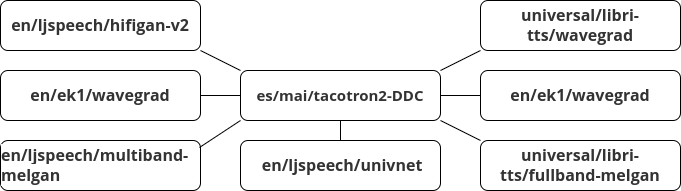
\includegraphics[width=0.7\linewidth]{Graphics/es_mai}
	\caption{Modelo TTS Tacotron2-DDC entrenado en Español}
	\label{esmai}
\end{figure}

\begin{figure}[H]
	\centering
	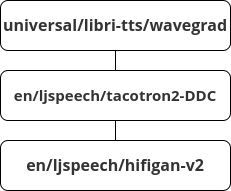
\includegraphics[width=0.3\linewidth]{Graphics/en_ljspeech}
	\caption{Modelo TTS Tacotron2-DDC entrenado en Inglés}
	\label{fig:enljspeech}
\end{figure}

\begin{figure}[H]
	\centering
	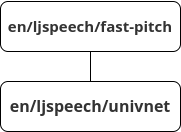
\includegraphics[width=0.3\linewidth]{Graphics/fastpitch}
	\caption{Modelo TTS Fast-Pitch entrenado en Inglés}
	\label{fig:fastpitch}
\end{figure}
\begin{figure}[H]
	\centering
	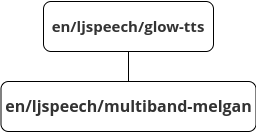
\includegraphics[width=0.4\linewidth]{Graphics/glow_tts}
	\caption{Modelo TTS Glow-TTS entrenado en Inglés}
	\label{fig:glowtts}
\end{figure}


Los modelos \textbf{Tacotron2-DDC, Fast-pitch y Glow-tts} preentrenados en idioma inglés al combinarse con VoCoders, como se observa en las figuras(citar figuras) para un texto en español arroja distintos resultados, en algunos casos solo producen ruido mientras que los más satisfactorios, producen un discurso con una pronunciación propia de una persona de habla inglesa hablando español.

Por otro lado Coqui solo cuenta con un modelo preentrenado en español, el \textbf{Tacontron-DDC}, que está entrenado sobre la base de datos de M-AILABS[\cite{mailabs}]; este modelo fue probado junto a los VoCoders preentrenados como se muestra en la figura \ref{esmai}. Los mejores resultados fueron arrojados por las combinaciones de \textbf{Tacontron-DDC} con los modelos: Univnet entrenado sobre la base de datos Ljspeech en inglés, y Wavegrad entrenado sobre el conjunto de datos LibriTTS, aunque ambos presentan problemáticas como la mala pronunciación de la letra ñ.\\

De acuerdo con la documentación de Coqui, y con el objetivo de la investigación que consiste en desarrollar un sintetizador de voz en español con voz cubana, se consideraron tres enfoques:

\begin{enumerate}
	\item Realizar un \textit{fine-tuning} o reentrenamiento a un modelo preentrenado de [\cite{coqui-doc}], en este caso \textbf{Tacontron-DDC}, que es el único disponible en español. 
	
	\item Realizar el entrenamiendo desde cero de un modelo; en este caso se podría entrenar cualquier modelo disponible. \textbf{Glow-TTS y VITS} son buenos candidatos pues en general producen resultados bastante satisfactorios.% Una desventaja es que cae una gran responsabilidad sobre el conjunto de datos de entrenamiento, pues debe tener una gran riqueza y muchos clips de audio.
	
	\item La problemática del tamaño de la base de datos puede resolverse entrenando el modelo \textbf{YourTTS}, que según la literatura, es capaz de adaptarse a una nueva voz con muy poco tiempo de audio.
\end{enumerate}

Para el desarrollo de cualquiera de los anteriores es imprescindible la construcción de un conjunto de datos que se adapten al modelo y a las necesidades de la investigación.


\section{Creación de la base de datos [\cite{formatting-dataset}]}

Para entrenar un modelo TTS, se necesita un conjunto de datos con grabaciones de voz y transcripciones, en este caso fue una base de datos en español con voces cubanas. El discurso debe dividirse en clips de audio y cada clip necesita su transcripción correspondiente. Debe poseer un formato específico de forma tal que el cargador de datos de Coqui TTS sea capaz de cargarlos para utilizar en el entrenamiento.    

La base de datos conformanda debe tener una buena cobertura del idioma en el que se desea entrenar el modelo. Debe cubrir la variedad fonémica, los sonidos excepcionales y las sílabas. 

\subsubsection{Qué hace a un buen Dataset?}

\begin{itemize}
	\item Debe cubrir una cantidad considerable de clips cortos y largos.
	\item Libre de errores. Se debe eliminar cualquier archivo incorrecto o roto. 
	\item Para escuchar una voz con la mayor naturalidad posible con todas las diferencias de frecuencia y tono, por ejemplo, usando diferentes signos de puntuación.
	\item Es necesario que el \textit{dataset} cubra una buena parte de fonemas, difonemas y, en algunos idiomas, trifonemas. Si la cobertura de fonemas es baja, el modelo puede tener dificultades para pronunciar nuevas palabras difíciles.
	
\end{itemize}

Los clips de audio poseen formato .wav y se organizan dentro de una carpeta de nombre \textit{wavs} de la siguiente forma:

\begin{center}
	/wavs\\
	| - audio1.wav\\
	| - audio1.wav\\
	| - audio2.wav\\
	| - audio3.wav\\
	...
\end{center}

Las transcripciones se recogen dentro del archivo metadata.csv. Donde audio1, audio2, etc se refieren a los archivos audio1.wav, audio2.wav etc.

\begin{center}
	audio1|Esta es mi transcripción 1.
	
	audio2|Esta es mi transcripción 2.
	
	audio3|Esta es mi transcripción 3.
	
	audio4|Esta es mi transcripción 4.
\end{center}

El modelo sobre el que realizaremos el ajuste, está preentrenado sobre la base de datos en Español de \textit{The M-AiLabs Speech Dataset}, por tanto utilizaremos la misma estructura de este en la conformación de la base de datos con voces cubanas. Finalmente queda la siguiente estructura:

\begin{flushleft}
	MyDataset/by$\_$book/female/[creador del dataset]/[nombre del hablante]
	
	|/wavs
	
	|metadata.csv
\end{flushleft}

\section{Reentrenamiendo para el ajuste de Tacontron-DDC}

Se propone desarrollar el primer enfoque: reentrenando(\textit{fine-tuning} en inglés) el modelo \textbf{Tacontron-DDC} en español, pues trae ventajas tales como un aprendizaje más rápido, ya que un modelo preentrenado ya tiene aprendidas funcionalidades que son relevantes para la tarea de producir un discurso. Convergerá más rápido en el nuevo \textit{dataset}, lo que reducirá el costo de entrenamiento y permitirá el proceso de experimentación más rápidamente. Además se pueden obtener buenos resultados con un conjunto de datos más pequeño.  \\

Luego de tener entrenado el modelo acústico(tts) con una base de datos construida con voces cubanas, es posible que alguno de los VoCoders preentrenados disponibles produzca una salida con las características deseadas, en caso contrario se debería entrenar el VoCoder con los datos del \textit{dataset} construido.

\subsection{Fine-Tuning}
Entrenar correctamente un modelo de aprendizaje profundo requiere generalmente de una gran base de datos y de un extenso entrenamiento.

Si se dispone del material necesario y del tiempo para entrenar el algoritmo, estos requisitos no suponen ningún problema, pero, si la base de datos es pequeña o el modelo no se entrena lo suficiente, el aprendizaje podría no ser completo.

El \textit{fine-tuning} es una forma de transferencia de aprendizaje, consiste en aprovechar la información que se ha aprendido de
la resolución de un problema y utilizarla sobre otro distinto, pero que comparte ciertas características. Se usan los conocimientos adquiridos por una red convolucional para transmitirlos a una nueva red convolucional. Esta nueva red convolucional que se crea no tiene por qué modificar la red original y puede simplemente aprender de ella, sin embargo también es válido el caso donde no solo se modifica la red original, sino que se vuelve a entrenar para aprender más conceptos.
  
En la presente investigación, se utiliza el reentrenamiento, para a partir modelo previamente entrenado y realizar un nuevo entrenamientor para mejorar su rendimiento en un conjunto de datos diferente.\\

El proceso consiste en modificar la configuración original del modelo preentrenado seleccionado, es decir, establecer la base de datos a utilizar en el reentrenamiento, los detalles acústicos que reflejen las características del nuevo conjunto de datos, el nombre del nuevo modelo ajustado, la dirección donde se guardará el modelo reentrenado, entre otras cuestiones. Para la mayoría de los parámetros se tomaron las características del modelo original \textbf{Tacontron-DDC} en español.



\section{Entrenamiento de modelo VITS desde cero}

Existen varios modelos de texto a voz de extremo a extremo que permiten el entrenamiento en una sola etapa y el muestreo en paralelo, sin embargo, generalmente la calidad de la muestra no coincide con la de los sistemas TTS de dos etapas. 

Se selecciona VITS porque es un método TTS paralelo de extremo a extremo que genera un sonido de audio más natural que los modelos actuales de dos etapas. Y de acuerdo a una evaluación humana subjetiva (puntuación de opinión media, o MOS), muestra que el modelo supera a los mejores sistemas TTS disponibles públicamente y logra un MOS comparable a la realidad del terreno.


	
	

%Are 100 audio samples sufficient?
%What should be the appropriate learning rate?
%What is the recommended length (no of characters) of each audio sample?
%Should we make any changes to batch size and number of epochs also? (Currently defaults in config file are 64 and 1000 respectively)
%Any other changes which should be done in the config.json file?
%Is tts_models--en--ljspeech--tacotron2-DDC_ph a good model to fine tune for custom voice?






